% In this last chapter an approach to the BCDI Phase Retrieval based on Automatic Differentiation will be discussed.
% It started from the necessity to 
% Unlke the DL model discussed above this method is iterative and

In this chapter a different approach to the BCDI phase retrieval will be presented. It originated from the need to resolve 
those cases in which neither standard alternating algorithms, nor the DL assisted PR can succeed to converge to a satisfactory 
reconstruction. The developed approach differs from the alternating projections algorithms classically used for 
the Fourier PR, as it is formulated as minimization problem solved with gradient descent (GD). The gradients however are computed 
through the efficient automatic differentiation (AD) enabled by graph-based differentiable programming packages like Tensorflow and 
PyTorch, accelerated on GPU. For this reason one could see the AD approach as unsupervised machine learning on a single training 
dataset.\\ 
The GD - based optimization is fundamentally different from fixed point alternating projections. Here one could qualitatively say 
that if the latter switches between real and reciprocal space applying constraints in both, the former initializes a 
complex object and updates at each cycle its modulus and phase using the gradients, with respect to them, of the differences 
between the observed and calculated diffracted intensities. In this way, the knowledge on the particle can be implemented 
by initializing the object with some physical constraints or adding regularization terms that will drive the updates 
towards more reasonable solutions. \\

After mentioning the most relevant literature on AD, and more generally GD-based, phase retrieval for CDI, 
we will present our formulation of the problem and the results obtained on simulated and experimental BCDI patterns. 

\section{State of the Art}
\section{Model implementation}
In an AD-driven optimization problem some trainable parameters are initialized. In the first basic formulation these 
trainable parameters can be the values of the voxels corresponding to the modulus $m$ and the phase $\varphi$ of the complex objects 
that represents the solution of the PR problem. All of these voxels contribute to the creation of a simulated 
diffracted intensity pattern via the forward model $I_{calc} = |\mathcal{F}\left\{ me^{i\varphi} \right\}|^2$. Subsequently, 
the gradients of a metric (loss function) that estimates the distance between the observed BCDI pattern $I_{obs}$ and $I_{calc}$ are calculated 
with respect to each of the trainable variables with automatic differentiation. At this point the value of each of these voxels is 
updated using a chosen optimizer (SGD, ADAM, etc.) and a given learning rate. The Tensorflow library allows for an easy 
implementation of the trainable variables and loss function and handles gradient operations with predefined methods. It is therefore 
straightforward to run the optimization as it follows the same structure of a deep learning model, with less trainable parameters and 
for a single data. 

However, such simple formulation of the complex object as mere real-valued variables is not optimal for a non-linear and non-convex 
inverse problem such the Fourier phase retrieval. In fact, many non-physical modulus-phase configuration could yield a 
$I_{calc}$ that is close to  $I_{obs}$. The presence of these local minima is the reason why, in conventional PR, algorithms 
like hybrid input-output, capable of escaping them, are employed. 
For this reason, the formulation of the complex object to be optimized has embedded some physical considerations that 
helped to restrict the solution space, removing some of the many local minima of populating the landscape of the BCDI PR. 
Moreover, it was shown by Marchesini in \cite{marchesini_unified_2007}
that steepest GD and the more sophisticated conjugate GD are more prone to get stuck in local 
minima, reason why they are not commonly utilized for Fourier PR. However, the active research field of machine learning has 
brought important advancements in the formulation of efficient and robust optimizers based on stochastic gradient descent with 
powerful features like Nesterov or adaptive momentum (ADAM \cite{ADAM}). These GD techniques are more robust to local minima, 
since the gradient is computed on mini-batches of trainable variables rather all of them (stochastic rather than classical steepest GD), 
and converge faster thanks to the ``memory'' of previous steps. Additionally, they are often wrapped into handy classes, ready to use, 
in Tensorflow and Pytorch libraries.  

\subsection{Object's shape}

The formulation of the object's shape has started considering the typical crystalline samples that are studied with the BCDI technique
and the requirements the modulus of the reconstructed object need to fulfill to be considered a ``good solution''. 
Usually, successful reconstruction show a \textit{homogeneous} modulus, sometimes quantitatively assessed through the 
mean-to-max metric \cite{Frisch2023CuAgCatalysts} , \cite{Grimes2024CatalystStrain}, as in standard BCDI the form factor is 
approximated uniform across all the scattering sites. Enforcing a homogeneous modulus by construction limits the search space 
and helps the convergence to the solution. 
It follows that parametrizing the \textit{surface} of the support, and setting to 1 the inside, is much more advantageous than optimizing 
the full 3D volume. This approach, already proposed by Scheinker and Pokharel in \cite{scheinker_adaptive_2020}, 
also significantly reduces the number of variables to optimize.

An additional consideration is that the probed samples are crystalline, thus often \textit{faceted} and \textit{convex}. 
Therefore, one could simplify even more the construction of the object shape by building a certain amount of planes in the 
3D space and obtain the support from the volume that lies inside the intersections of all them. This would remove the possibility 
to have spikes or rough surfaces that might satisfy some local minimum but wouldn't represent a crystal. Moreover, with this 
representation the number of trainable variables would be further reduced. 

According to this scheme the relevant parameters to be optimized are the angles $\theta$ and $ \varphi$ of the spherical 
coordinates and the length $d$ of a given number $N$ of the so-called \textit{half-spaces}. 
More formally, the normals $n_i$ for each of the $N$ half-spaces are defined with a pair of ($\theta , \varphi$) that  its
orientation in space (Eq. \ref{eq:normal_vector}). Subsequently, only the intersection of those $(x,y,z)$ coordinates for which the dot product with 
each $n_i$ is smaller than the length $d_i$ is considered as support (Eq. \ref{eq:convex_hull}).


\begin{equation}
    \mathbf n_i \;=\;
    \begin{pmatrix}
    \sin\varphi_i\cos\theta_i \\[6pt]
    \sin\varphi_i\sin\theta_i \\[6pt]
    \cos\varphi_i
    \end{pmatrix},
    \label{eq:normal_vector}
    \end{equation}
    
    \begin{equation}
    \mathcal S \;=\;
    \bigcap_{i=1}^N
    \Bigl\{\mathbf x=(x,y,z)\in\mathbb R^3 : 
    \mathbf n_i\cdot\mathbf x \le d_i\Bigr\},
    \label{eq:convex_hull}
    \end{equation}

A schematic representation of this construction is provided by Fig. \ref{fig:support_construction}.
 
With this approach the user needs to provide a number of half-spaces as hyperpareter meaning that a sort of prior knowledge 
on the sample can be leveraged in these regards as well. However, this number doesn't have to be precisely the number of 
facets expected. In fact, a large $N$ is often advised for unknown sample shape such that even roundish objects can be 
retrieved. In case of well faceted samples the large $N$ is a minor problem as many $n_i$ will be automatically aligned to the 
same $(\theta_i, \varphi_i, d_i)$ at the cost of some more trainable parameters. 

\begin{figure}[H]
    \centering
    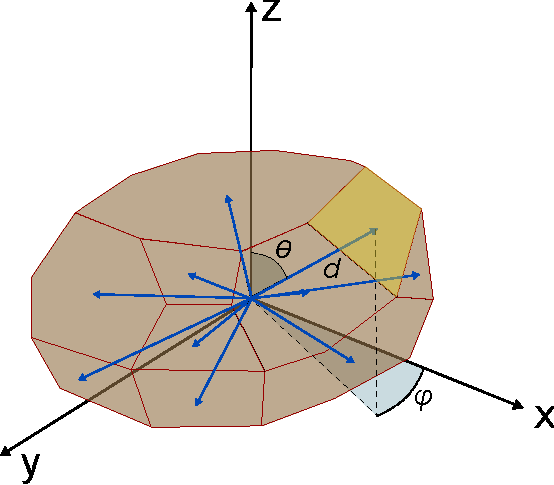
\includegraphics[width=.8\textwidth]{figures/AD/AD.pdf}
    \caption{Construction of the convex hull with half-spaces expressed with spherical coordinates }
    \label{fig:support_construction}
\end{figure}

The last important consideration of this parametrization is that the support $\mathcal S$ is sharply divided into a binary 
variable (1 inside and 0 outside) thus leading to differentiability problems. In fact, in such a way the gradients, essential for the 
support update, are not defined. For this reason $\mathcal S$ is first passed through a sigmoid function controlled by an 
hyperparameter $eps$ responsible for the smoothening of the support borders. This measure can also be seen as a control of the 
resolution of the object. 

\subsection{Object's phase}

\subsection{Loss function}

\section{Results}
\subsection{Low-strain case}
\subsection{High-strain case}
\section{Conclusions}
